\chapter{Error Handling}
\label{ch:error_handling}

Software systems constantly interact with unpredictable environments: networks drop, disks fill up, files are locked by other processes, and users provide invalid input. Robust professional software is not defined merely by its ability to execute the "happy path," but by its resilience and predictability when failures occur. 

In this chapter, we explore how Rust models and manages errors. By treating errors as standard data types and leveraging the type system, Rust forces developers to acknowledge failures without sacrificing code readability.

\section{The Taxonomy of Failures: Recoverable vs. Unrecoverable}

When an operation fails, we must determine if the program can gracefully recover. Failures generally fall into two categories:

\begin{itemize}
    \item \textbf{Unrecoverable Errors:} These occur when a fundamental invariant of the program is broken, or a catastrophic resource constraint is hit (e.g., Out of Memory, Stack Overflow). For instance, accessing an array out of bounds implies a logic bug. In these scenarios, the safest action is to immediately halt execution to prevent data corruption.
    \item \textbf{Recoverable Errors:} These arise from temporary or external conditions, such as attempting to read a missing configuration file, dealing with a locked file, or failing to connect to a database. The program should anticipate these. Common recovery strategies include:
    \begin{itemize}
        \item \textbf{Exponential Backoff:} When a network server is unreachable, wait 100ms, then 200ms, 400ms, 800ms, up to a sensible maximum to gracefully retry without overwhelming the system. Be careful to avoid infinite loops.
        \item \textbf{Skip and Continue:} If reading a file and a specific line (e.g., line 27) is corrupted, log the error and continue processing the next lines.
        \item \textbf{Default Values:} If a configuration file is missing, fallback to sensible default settings.
        \item \textbf{User Intervention:} If the application is interactive (attached to a console), prompt the user for alternative input. If running in batch mode (e.g., standard input via a pipe), abort or log the failure instead.
    \end{itemize}
\end{itemize}

\begin{examprioritybox}
\textbf{The Database Analogy (ACID Properties)}\\
Consider how a Database Management System (DBMS) handles failures. If a disk fills up mid-transaction, the DBMS does not corrupt the data; it rolls back to a valid, consistent state. This is governed by ACID properties:
\begin{itemize}
    \item \textbf{Atomicity:} The entire transaction either succeeds or fails.
    \item \textbf{Consistency:} The database moves from one valid state to another (e.g., referential integrity is maintained, non-null and unique constraints are respected).
    \item \textbf{Isolation:} Intermediate states during a transaction are invisible to other operations.
    \item \textbf{Durability:} Once committed, the changes remain permanently.
\end{itemize}
Professional software should mimic this resilience, managing side-effects and ensuring predictable state transitions even when individual operations fail.

\textbf{Common Pitfall:} Treating file operations like guaranteed database transactions without manually handling partial writes or state corruption on failure (e.g., a file write fails halfway through because the disk is full).

\textbf{Expected Mastery Level:} Deep conceptual understanding; you should be able to explain how error handling in Rust provides similar guarantees to database ACID properties.
\end{examprioritybox}

\section{Unrecoverable Errors and Panics}

When an unrecoverable error occurs, Rust provides the \texttt{panic!} macro. Invoking a panic immediately halts the current thread's normal execution flow.

\begin{lstlisting}[language=Rust]
fn main() {
    let device_id = 42;
    panic!("A critical hardware failure occurred on device {}. Aborting.", device_id);
}
\end{lstlisting}

Just like \texttt{println!}, the \texttt{panic!} macro accepts formatting placeholders to build detailed, context-rich error messages.

By default, panicking initiates \emph{stack unwinding}. Rust walks back up the call stack, cleaning up variables, calling destructors, and freeing memory cleanly. Alternatively, a panic can be configured at compile time to immediately \emph{abort} the process, leaving the cleanup to the operating system.

\begin{warningbox}
\textbf{Panic vs. Process Exit}\\
There is a crucial difference between panicking and forcefully exiting via \texttt{std::process::exit(code)}. Invoking \texttt{exit()} immediately terminates the program without running any destructors, akin to sending a \texttt{kill -9} signal to the process from the OS. In contrast, \texttt{panic!} safely unwinds the stack. Avoid \texttt{exit()} unless you specifically intend to bypass cleanup.
\end{warningbox}

Another useful macro is \texttt{unreachable!()}. We use it to mark execution paths that we, the developers, know are logically impossible, even if the compiler cannot prove it. If an \texttt{unreachable!()} is ever executed, it immediately triggers a panic.

\begin{warningbox}
Do not use \texttt{panic!} for standard control flow or predictable environmental errors. A library function should never panic on bad user input; it should return a structured error instead, leaving the decision to halt up to the application developer.
\end{warningbox}

\section{Enums, Structs, and Pattern Matching}

Before diving into Rust's primary error structures, we must briefly revisit Enums and pattern matching, as they form the foundation of error handling.

In Rust, Enums are \emph{Sum Types}. From a mathematical perspective, the domain of an enum is the union of the domains of its variants. They can represent entirely distinct alternatives and encapsulate data within those alternatives.

\begin{lstlisting}[language=Rust]
enum Shape {
    Square(f64),
    Circle(f64),
}

impl Shape {
    fn area(&self) -> f64 {
        match self {
            Shape::Square(s) => s * s,
            Shape::Circle(r) => r * r * std::f64::consts::PI,
        }
    }
}
\end{lstlisting}

\begin{memoryblock}
\textbf{Memory Layout of Enums:}\\
Internally, an enum requires memory for a \emph{discriminant} (a tag indicating which variant is currently active, typically at least 1 byte) plus the space required for its largest variant. For instance, if an enum has a \texttt{Square(f64)} variant requiring 8 bytes, the enum will take 1 byte for the tag plus 8 bytes for the data. Due to memory alignment rules, this usually pads the total size to 16 bytes.

When destructuring an enum via \texttt{match}, the enum is consumed. If passed by value, its stack memory is reclaimed once the function returns.
\end{memoryblock}

\textbf{When and why to use it:} Use \texttt{match} when you need exhaustive checking over all possible variants of an Enum. The compiler will enforce that every variant is accounted for, making refactoring much safer.

\subsection{Selective Destructuring with \texttt{if let} and \texttt{while let}}

When we only care about extracting data from a single variant, writing a full \texttt{match} block with a catch-all \texttt{\_ => ()} arm can be verbose. Rust provides the \texttt{if let} construct for targeted destructuring.

\begin{lstlisting}[language=Rust]
let shape = Shape::Square(5.0);
if let Shape::Square(s) = shape {
    println!("Found a square with side: {}", s);
}
\end{lstlisting}

This code attempts to assign the value inside \texttt{shape} to the variable \texttt{s}. If \texttt{shape} is indeed a \texttt{Square}, the block executes. Because this operation involves a move assignment (unless references are used), the original \texttt{shape} is dismantled and becomes inaccessible after this block.

\begin{insightbox}
\textbf{Enums as Monads}\\
In the functional theory of types, an Enum in this context acts as a \emph{monad}. It is a container that safely encapsulates varying internal details depending on the specific variant. By providing controlled mechanisms to "unpack" this container (like \texttt{if let}), Rust forces you to handle the encapsulated state safely.
\end{insightbox}

Similarly, \texttt{while let} can be used to continuously pull values out of an Enum until it fails. This is highly useful when reading lines from a file sequentially:

\begin{lstlisting}[language=Rust]
while let Ok(line) = reader.read_line() {
    // Process line
}
\end{lstlisting}

\subsection{Struct Destructuring}

While enums represent alternative variants requiring conditional destructuring (hence \texttt{if let}), Structs do not have ambiguity. We know exactly what fields a struct possesses, so destructuring never fails:

\begin{lstlisting}[language=Rust]
struct Point { x: f64, y: f64 }
let p = Point { x: 1.0, y: 2.0 };

// Infallible destructuring
let Point { x, y } = p; 
\end{lstlisting}

This syntax avoids the repetitive boilerplate of writing \texttt{p.x} and \texttt{p.y}. Note that destructuring a struct follows standard move semantics: if the struct implements the \texttt{Copy} trait, the original remains usable; otherwise, ownership of the fields transfers to the new variables, rendering the original struct inaccessible. (Note: Modern Rust 2024 editions simplify retaining references during destructuring).

\section{Recoverable Errors: \texttt{Result} and \texttt{Option}}

Historically, languages like C handled recoverable errors by returning special integer codes (e.g., returning \texttt{0} for success or \texttt{-1} for failure). This approach is flawed because the compiler cannot force the developer to check the return code. 

Languages like Java and C++ introduced Exceptions, which enforce error handling but hide the control flow. In Java, exceptions were split into \texttt{Error} (unrecoverable catastrophic failures like \texttt{OutOfMemoryError} or \texttt{StackOverflowError} where the JVM breaks) and \texttt{Exception} (recoverable). \textit{Checked exceptions} forced developers to handle errors, but often led to unreadable boilerplate (such as deep \texttt{catch} blocks), pushing many towards unchecked \texttt{RuntimeException}s. Furthermore, the superstructure required to manage the call stack and context switching for exception handling is costly. This is a primary reason why C++ exceptions cannot be used when writing Linux kernel modules, as they break the kernel's execution assumptions. 

Rust avoids implicit exception throwing, solving this instead using standard Enums. The two primary types for representing optionality and errors are \texttt{Option<T>} and \texttt{Result<T, E>}.

\begin{lstlisting}[language=Rust]
enum Option<T> {
    Some(T),
    None,
}

enum Result<T, E> {
    Ok(T),
    Err(E),
}
\end{lstlisting}

The \texttt{Option} enum represents the presence (\texttt{Some}) or absence (\texttt{None}) of a value. It is ideal when the \emph{reason} for absence is obvious or irrelevant. 

The \texttt{Result} enum is more expressive. It represents either a successful outcome containing a value of type \texttt{T}, or a failure containing an error of type \texttt{E}. Because \texttt{Result} is a standard return type, it explicitly signals in the function signature that an operation can fail.

\begin{figure}[h]
    \centering
    % AI-IMAGE-REQUEST: A flowchart showing a function returning a Result branching into Ok(value) continuing execution and Err(error) diverting to an error handling path.
    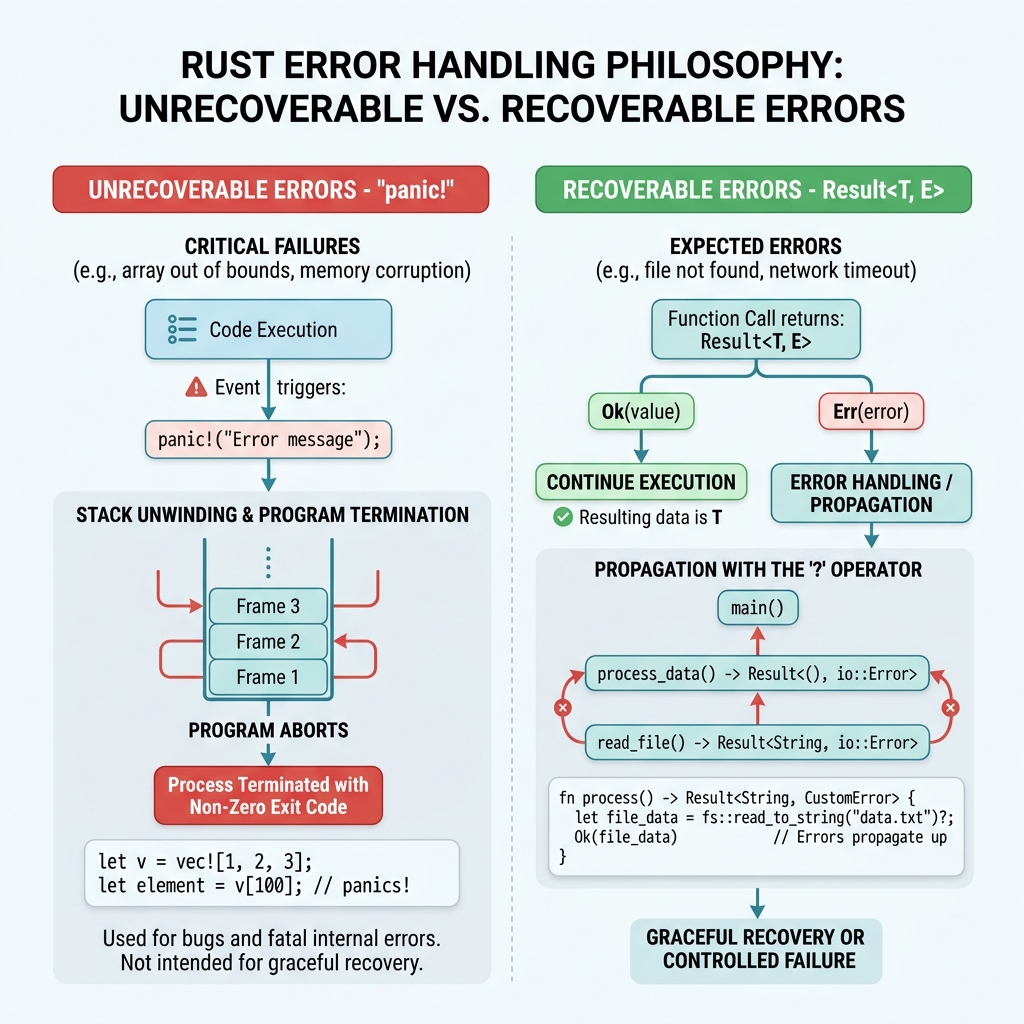
\includegraphics[width=0.8\textwidth]{images/error_handling.png}
    \caption{Conceptual model of Error Handling with Result in Rust.}
    \label{fig:error_handling}
\end{figure}

\subsection{Extracting Values and Handling Errors}

When a function returns a \texttt{Result}, you must explicitly handle it. The most exhaustive method is using a \texttt{match} block.

\begin{lstlisting}[language=Rust]
use std::fs::File;

let file_result = File::open("config.txt");

let file = match file_result {
    Ok(f) => f,
    Err(e) => {
        println!("Failed to open file: {}", e);
        return;
    }
};
\end{lstlisting}

\begin{memoryblock}
The \texttt{File::open} call asks the OS to allocate a file descriptor, and it returns a \texttt{Result<File, std::io::Error>} enum allocated on the stack. The \texttt{match} expression consumes this \texttt{Result} by value. If it is \texttt{Ok}, ownership of the \texttt{File} struct is moved into the \texttt{file} variable. If it is \texttt{Err}, the error \texttt{e} is captured by value, printed, and the function returns early. Since \texttt{Result} transfers ownership, \texttt{file\_result} is invalid and inaccessible after the \texttt{match} block.
\end{memoryblock}

Rust also provides a suite of helper methods on \texttt{Result} and \texttt{Option}:
\begin{itemize}
    \item \textbf{\texttt{is\_ok()} / \texttt{is\_err()}:} Returns a boolean indicating the variant.
    \item \textbf{\texttt{map()}:} Applies a function to the inner value if it is \texttt{Ok} or \texttt{Some}, leaving errors untouched.
    \item \textbf{\texttt{contains(\&x)}:} Returns true if the result is successful and contains a value that exactly matches the provided argument \texttt{x}.
\end{itemize}

\begin{notebox}
The \texttt{ok()} and \texttt{err()} methods are extremely useful for converting between \texttt{Result} and \texttt{Option}. Calling \texttt{ok()} on a \texttt{Result} returns \texttt{Some(value)} if it was successful, and \texttt{None} if it was an error, effectively discarding the error details when you no longer need them. Conversely, you can convert an \texttt{Option} into a \texttt{Result} using \texttt{ok\_or()}.
\end{notebox}

For rapid prototyping, you might see \texttt{unwrap()} or \texttt{expect()}.
\begin{lstlisting}[language=Rust]
// Panics if the result is an Err
let file = File::open("config.txt").unwrap(); 

// Panics with a custom message
let file = File::open("config.txt").expect("config.txt must exist!");
\end{lstlisting}

\begin{examprioritybox}
\textbf{The Danger of unwrap() and expect()}\\
Using \texttt{unwrap()} explicitly converts a recoverable error (\texttt{Result}) into an unrecoverable error (\texttt{panic!}). In professional code, \texttt{unwrap()} should be avoided unless you are absolutely certain the operation cannot fail (e.g. proving an invariant). Panicking initiates stack unwinding or aborts the process entirely, potentially leaving external resources or shared state in an inconsistent state.

\textbf{Common Pitfall:} Using \texttt{unwrap()} in production code for convenience, resulting in unexpected application crashes when an environment changes (like a missing file or a network drop).

\textbf{Expected Mastery Level:} High. You must confidently distinguish between a recoverable failure (to be handled via \texttt{Result} and \texttt{?}) and an unrecoverable failure (where \texttt{unwrap} or \texttt{panic!} is semantically correct).
\end{examprioritybox}

\section{The Happy Path: The \texttt{?} Operator}

Handling every error manually with \texttt{match} drastically increases cyclomatic complexity. Our code becomes deeply nested, obscuring the primary logic (the "Happy Path"). 

Often, a function doesn't know how to handle an error; it simply needs to propagate it up to the caller. Rust provides the \texttt{?} (question mark) operator to automate this boilerplate.

Consider this verbose function:

\begin{lstlisting}[language=Rust]
use std::fs::File;
use std::io::Read;

fn read_file_verbose(name: &str) -> Result<String, std::io::Error> {
    let mut file = match File::open(name) {
        Ok(f) => f,
        Err(e) => return Err(e), // Early return on error
    };
    
    let mut s = String::new();
    match file.read_to_string(&mut s) {
        Ok(_) => Ok(s),
        Err(e) => Err(e),
    }
}
\end{lstlisting}

The \texttt{?} operator can be placed after any expression returning a \texttt{Result}. If the value is \texttt{Ok}, it unwraps the inner value and execution continues. If the value is \texttt{Err}, it \emph{immediately returns} from the entire function, passing the error to the caller.

Here is the exact same logic written idiomatically:

\begin{lstlisting}[language=Rust]
fn read_file(name: &str) -> Result<String, std::io::Error> {
    let mut file = File::open(name)?;
    let mut s = String::new();
    file.read_to_string(&mut s)?;
    Ok(s)
}
\end{lstlisting}

\begin{memoryblock}
\texttt{name} is a borrowed string slice (\texttt{\&str}), meaning it points to string data managed elsewhere without taking ownership. \texttt{File::open} returns a \texttt{Result} on the stack. The \texttt{?} operator consumes it: on success, the \texttt{File} struct's ownership is moved to \texttt{file}. \texttt{String::new()} allocates a string struct on the stack with a pointer to an initially empty heap buffer. \texttt{read\_to\_string} mutably borrows \texttt{s} (\texttt{\&mut s}), enabling it to dynamically resize the heap buffer to fit the file contents. Finally, \texttt{Ok(s)} takes ownership of \texttt{s} and transfers it back to the caller wrapped in a \texttt{Result}, seamlessly preserving the heap-allocated buffer.
\end{memoryblock}

\textbf{When and why to use it:} The \texttt{?} operator should be your default choice for propagating errors. It flattens the "Happy Path" and delegates error handling to higher levels in the call stack where more context is available.

\begin{insightbox}
\textbf{The Power of the \texttt{?} Operator}\\
The \texttt{?} operator is not just syntactic sugar; it defines the visual flow of Rust code. It keeps the core logic flat and readable while maintaining strict type safety. Notice that any function using the \texttt{?} operator must itself have a return type compatible with the error being propagated (e.g., returning a \texttt{Result}).
\end{insightbox}

\section{Handling Heterogeneous Errors}

A significant challenge arises when a single function performs operations that produce \emph{different} error types. For example, reading a file produces an \texttt{std::io::Error}, but parsing its string contents into an integer produces an \texttt{std::num::ParseIntError}. 

\begin{lstlisting}[language=Rust]
use std::fs::File;
use std::io::{self, BufRead};

// What should the Return Type be? 
// We have two incompatible Error types!
fn sum_file(name: &str) -> Result<i32, ???> {
    let file = File::open(name)?; // io::Error
    let reader = io::BufReader::new(file);
    let mut sum = 0;
    
    for line in reader.lines() {
        let line = line.unwrap(); // Using unwrap to avoid type mismatch
        let num: i32 = line.parse()?; // ParseIntError
        sum += num;
    }
    
    Ok(sum)
}
\end{lstlisting}

We cannot place two different types in the \texttt{E} generic parameter of a standard \texttt{Result}. There are three primary ways to solve this gracefully.

\subsection{Trait Objects: \texttt{Box<dyn Error>}}

We can use polymorphism by returning a pointer to \emph{any} type that implements the \texttt{Error} trait. 

\begin{lstlisting}[language=Rust]
use std::error::Error;

fn sum_file(name: &str) -> Result<i32, Box<dyn Error>> {
    let file = File::open(name)?;
    let reader = io::BufReader::new(file);
    let mut sum = 0;
    
    for line in reader.lines() {
        let line = line?; // Works automatically!
        let num: i32 = line.parse()?; // Works automatically!
        sum += num;
    }
    
    Ok(sum)
}
\end{lstlisting}

\begin{memoryblock}
Returning \texttt{Box<dyn Error>} triggers a heap allocation if an error occurs. The specific error struct (like \texttt{std::io::Error} or \texttt{std::num::ParseIntError}) is allocated and moved onto the heap. A \textit{fat pointer} (comprising a data pointer and a vtable pointer for dynamic dispatch) is returned on the stack inside the \texttt{Result::Err}. While this provides extreme flexibility for polymorphic error handling, it incurs the runtime cost of memory allocation and pointer indirection, unlike generic \texttt{Result<T, E>} objects which reside entirely on the stack.
\end{memoryblock}

The \texttt{?} operator automatically converts specific errors (like \texttt{io::Error}) into a heap-allocated \texttt{Box<dyn Error>} by leveraging the standard library's implementation of the \texttt{From} trait. While highly flexible, the caller loses compile-time knowledge of exactly which errors can occur. 

To handle specific errors dynamically, the caller must use \emph{downcasting}:

\begin{lstlisting}[language=Rust]
fn handle_sumfile_errors(name: &str) {
    match sum_file(name) {
        Ok(sum) => println!("The sum is: {}", sum),
        Err(e) => {
            if let Some(io_err) = e.downcast_ref::<io::Error>() {
                println!("Disk/Network failure: {}", io_err);
            } else if let Some(parse_err) = e.downcast_ref::<std::num::ParseIntError>() {
                println!("Invalid number format: {}", parse_err);
            } else {
                unreachable!("Unexpected error type!");
            }
        }
    }
}
\end{lstlisting}

\subsection{Custom Enums}

For rigorous domains, creating a custom Enum to unify the errors is the most robust approach.

\begin{lstlisting}[language=Rust]
enum SumFileError {
    Io(std::io::Error),
    Parse(std::num::ParseIntError),
}
\end{lstlisting}

This gives the caller exhaustive, type-safe matching without needing dynamic dispatch. However, manually writing the conversion boilerplate to allow the \texttt{?} operator to seamlessly cast \texttt{io::Error} into \texttt{SumFileError::Io} can be tedious.

\subsection{Ecosystem Solutions: \texttt{thiserror} and \texttt{anyhow}}

Because managing heterogeneous errors is so common, the Rust ecosystem relies heavily on two community crates:

\begin{itemize}
    \item \textbf{\texttt{thiserror}:} Used when writing \emph{Libraries}. By simply adding the \texttt{\#[derive(Error, Debug)]} attribute, and annotating Enum variants with \texttt{\#[error("...")]} and \texttt{\#[from]}, it automatically implements the \texttt{Error}, \texttt{Display}, and \texttt{From} traits. This allows you to elegantly expose strict, structured errors to your users as part of your library's API contract.
    \item \textbf{\texttt{anyhow}:} Used when writing \emph{Applications}, where code simplicity takes priority over strict error type inspection. It provides a smart \texttt{anyhow::Result} type that transparently absorbs any error implementing the \texttt{Error} trait. It allows you to attach custom contextual strings to explain what the code was trying to do when the failure occurred (e.g., \texttt{file.read().context("Failed to read config")} or \texttt{.with\_context(|| format!("Missing path \{\}", path))}), and handles stack traces gracefully.
\end{itemize}

\begin{examprioritybox}
\textbf{Handling Heterogeneous Errors}\\
Be prepared to identify why a function containing multiple \texttt{?} operators fails to compile due to mismatched error types. Use custom Enums (or \texttt{thiserror}) when you need the caller to meticulously inspect and recover from specific errors; use \texttt{Box<dyn Error>} (or \texttt{anyhow}) when you simply want to propagate a formatted error trace and abort or log it.

\textbf{Common Pitfall:} Misunderstanding the performance and API consequences of \texttt{Box<dyn Error>}. While easy to write, it hides error types from the compiler, making strict error recovery tedious and requiring manual downcasting.

\textbf{Expected Mastery Level:} Very High. You must be able to recognize heterogeneous errors and implement both a custom enum wrapper and a dynamic dispatch approach.
\end{examprioritybox}

\section*{Further Reading}

To deepen your understanding of error handling in Rust, the following resources (recommended in the lectures) are highly valuable:
\begin{itemize}
    \item \href{https://medium.com/coinmonks/rust-error-handling-in-practice-376d86ba12ca}{Rust Error Handling In Practice}: A solid overview of basic error management concepts with practical examples.
    \item \href{https://kerkour.com/rust-error-handling}{The simplest guide to error handling in Rust}: A hands-on guide focusing heavily on how to structure errors using the \texttt{thiserror} and \texttt{anyhow} crates.
    \item \href{https://www.learnrust.blog/p/idiomatic-error-handling-in-rust}{Idiomatic Error Handling in Rust}: Another practical approach to applying Rust's patterns idiomatically.
    \item \href{https://www.lpalmieri.com/posts/error-handling-rust/}{Error Handling In Rust - A Deep Dive}: An excerpt from the book \textit{"Zero To Production In Rust"} that explores advanced error management in real-world scenarios.
\end{itemize}



\subsection*{Exam Relevance and Recurrence}
\textbf{Score:} Very High \\
\textbf{Notes:} Error handling is guaranteed to appear in exams. You will likely be asked to refactor verbose code using \texttt{match} into idiomatic code using the \texttt{?} operator. Questions frequently cover the implications of using \texttt{unwrap()}, memory models and cost differences between \texttt{Box<dyn Error>} and custom Enums, and identifying missing implementations to allow the \texttt{?} operator to seamlessly cast errors.

\section{Domande ed Esercizi da Esami Passati}

\begin{exambox}
\textbf{Domanda 1}
\begin{enumerate}
    \item Si descriva il meccanismo di gestione degli errori fornito dal linguaggio RUST, differenziando tra quelli recuperabili e irrecuperabili
    \item Si spieghi il funzionamento dell'operatore ?
    \item Si mostri un esempio di applicazione dell'operatore ? scrivendo una funzione (avendo cura di scriverla completamente) che deve cercare una stringa (my\_string) e restituire il suo offset in un file, se presente.
\end{enumerate}

\textbf{Soluzione:}
\begin{enumerate}
    \item In Rust, la gestione degli errori distingue tra due categorie principali:
    \begin{itemize}
        \item \textbf{Errori irrecuperabili:} si verificano quando vengono violate invarianti fondamentali (es. accesso fuori dai limiti di un array) o per vincoli insuperabili. Vengono gestiti tramite la macro \texttt{panic!} (o \texttt{unreachable!()}), che interrompe immediatamente l'esecuzione del thread corrente ed esegue lo \textit{stack unwinding} per liberare la memoria in modo sicuro.
        \item \textbf{Errori recuperabili:} sono fallimenti prevedibili legati all'ambiente (es. file mancante). Rust non usa eccezioni implicite, ma si affida ai tipi \texttt{Result<T, E>} e \texttt{Option<T>}. Il compilatore forza lo sviluppatore a gestire esplicitamente questi scenari, ad esempio tramite costrutti di pattern matching come \texttt{match} o \texttt{if let}.
    \end{itemize}
    \item L'operatore \texttt{?} è uno strumento idiomatico per propagare gli errori, riducendo la verbosità del codice (\textit{boilerplate} dei blocchi \texttt{match}). Posizionato dopo un'espressione che restituisce un \texttt{Result}, se il risultato è \texttt{Ok(T)}, l'operatore estrae il valore interno \texttt{T} permettendo all'esecuzione di continuare; se il risultato è \texttt{Err(E)}, la funzione termina immediatamente restituendo l'errore al chiamante. L'operatore gestisce anche conversioni automatiche di tipi di errore compatibili.
    \item Esempio di applicazione dell'operatore \texttt{?} per la ricerca di una stringa in un file:
\begin{lstlisting}[language=Rust]
use std::fs::File;
use std::io::{self, Read};

fn find_string_offset(name: &str, my_string: &str) -> Result<Option<usize>, io::Error> {
    let mut file = File::open(name)?; // Propaga l'errore se il file non esiste
    let mut contents = String::new();
    file.read_to_string(&mut contents)?; // Propaga l'errore se la lettura fallisce
    
    Ok(contents.find(my_string)) // Restituisce l'offset avvolto in Result::Ok
}
\end{lstlisting}
\end{enumerate}
\end{exambox}

\begin{exambox}
\textbf{Domanda 2}\\
Si illustri come sia possibile gestire correttamente le situazioni di errore in Rust, distinguendo tra Option e Result.

\textbf{Soluzione:}\\
In Rust, gli errori recuperabili vengono gestiti evitando le eccezioni implicite e utilizzando due Enum standard:
\begin{itemize}
    \item \textbf{\texttt{Option<T>}:} rappresenta la presenza (\texttt{Some(T)}) o l'assenza (\texttt{None}) di un valore. È la scelta ideale quando il motivo del fallimento o dell'assenza del dato è ovvio o irrilevante.
    \item \textbf{\texttt{Result<T, E>}:} è un'astrazione più espressiva che rappresenta un esito di successo con il valore associato (\texttt{Ok(T)}) o un fallimento con l'errore associato (\texttt{Err(E)}). Includendo esplicitamente il potenziale fallimento nella \textit{signature} della funzione, il compilatore costringe a gestire entrambi i casi.
\end{itemize}
Queste strutture devono essere gestite in modo esplicito (es. con \texttt{match}, \texttt{if let} o l'operatore \texttt{?}). Esistono inoltre vari metodi di utilità come \texttt{ok()} ed \texttt{err()} che permettono di convertire agevolmente un \texttt{Result} in un \texttt{Option}, scartando i dettagli dell'errore. L'uso di funzioni come \texttt{unwrap()} è invece sconsigliato in produzione, poiché converte tali errori recuperabili in errori irrecuperabili causando un \texttt{panic!} e arrestando l'esecuzione del programma.
\end{exambox}
